\documentclass[tikz, border=0pt]{standalone}
\usepackage{fontspec}
\setmainfont{Latin Modern Mono}
\usepackage{tikz}
\usetikzlibrary{arrows.meta, positioning, calc, fit, backgrounds}

% ---------- Minimal dark palette (GitHub-dark inspired, restrained) ----------
\definecolor{bg}{HTML}{0D1117}
\definecolor{line}{HTML}{30363D}
\definecolor{lineSoft}{HTML}{21262D}
\definecolor{accent}{HTML}{C9A227}   % used once, only to mark the LLM box
\definecolor{txt}{HTML}{C9D1D9}
\definecolor{txtDim}{HTML}{6E7681}
\definecolor{arrow}{HTML}{484F58}

\tikzset{
  node/.style={
    rectangle, draw=line, line width=0.6pt, rounded corners=1pt,
    minimum width=7.2cm, minimum height=1.15cm, align=center,
    fill=bg, font=\small, text=txt
  },
  smallnode/.style={
    rectangle, draw=line, line width=0.6pt, rounded corners=1pt,
    minimum width=4.55cm, minimum height=1.15cm, align=center,
    fill=bg, font=\scriptsize, text=txt
  },
  arr/.style={-{Stealth[length=1.8mm, width=1.3mm]}, line width=0.6pt, draw=arrow},
  label/.style={font=\scriptsize, text=txtDim}
}

\begin{document}
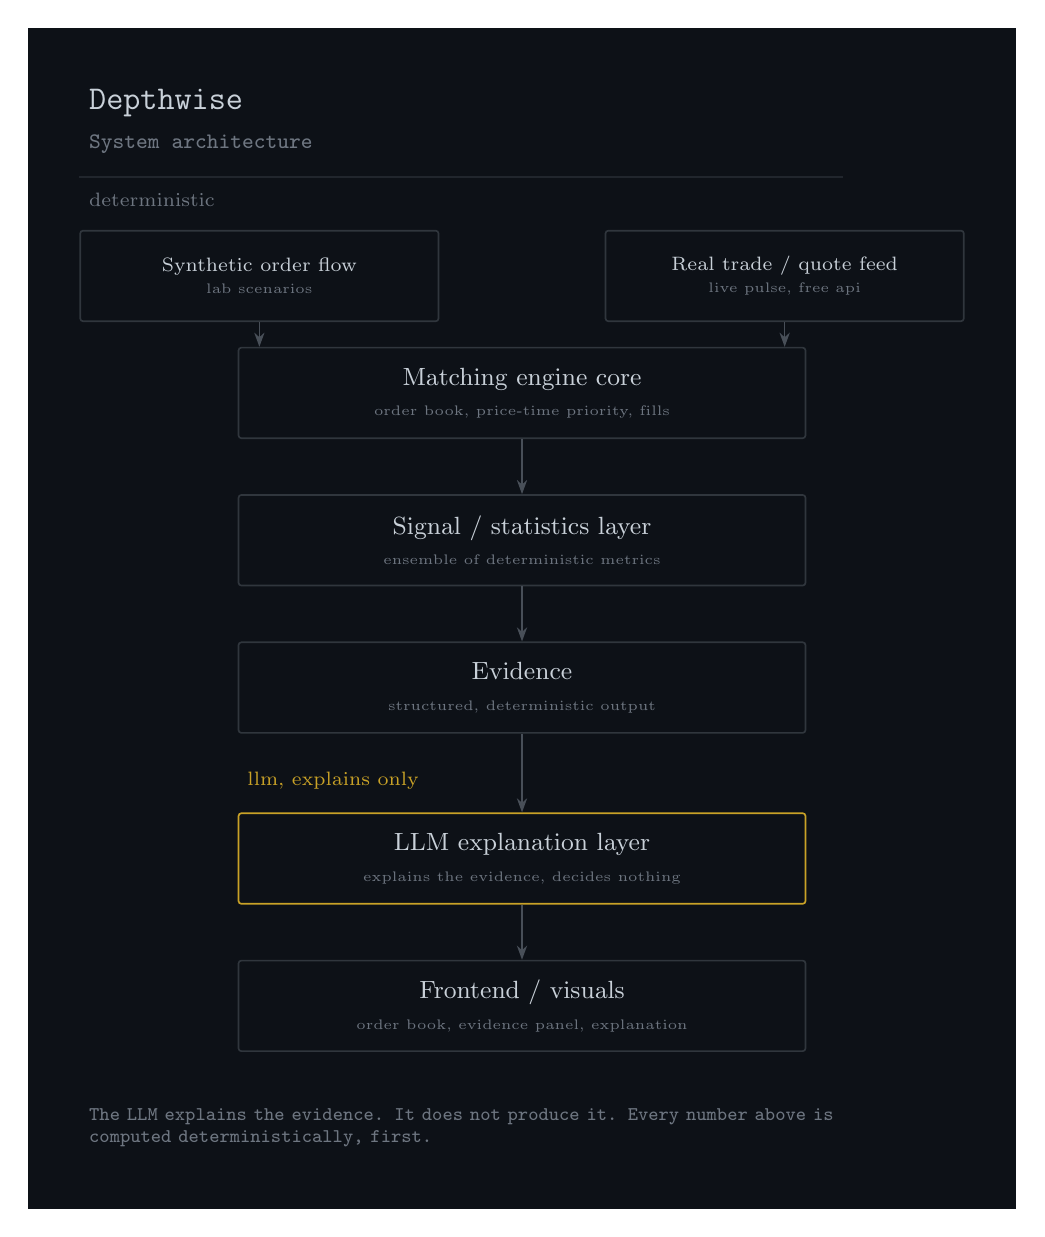
\begin{tikzpicture}[node distance=0.55cm, font=\ttfamily]

% ---------------- Pipeline ----------------
\node[smallnode] (synth) {Synthetic order flow\\\tiny\color{txtDim} lab scenarios};
\node[smallnode, right=2.1cm of synth] (real) {Real trade / quote feed\\\tiny\color{txtDim} live pulse, free api};

\node[node, below=0.9cm of $(synth)!0.5!(real)$] (matching) {Matching engine core\\\tiny\color{txtDim} order book, price-time priority, fills};
\node[node, below=0.7cm of matching] (signal) {Signal / statistics layer\\\tiny\color{txtDim} ensemble of deterministic metrics};
\node[node, below=0.7cm of signal] (evidence) {Evidence\\\tiny\color{txtDim} structured, deterministic output};
\node[node, draw=accent, below=1.0cm of evidence] (llm) {LLM explanation layer\\\tiny\color{txtDim} explains the evidence, decides nothing};
\node[node, below=0.7cm of llm] (frontend) {Frontend / visuals\\\tiny\color{txtDim} order book, evidence panel, explanation};

\draw[arr] (synth.south) -- (synth |- matching.north);
\draw[arr] (real.south) -- (real |- matching.north);
\draw[arr] (matching) -- (signal);
\draw[arr] (signal) -- (evidence);
\draw[arr] (evidence) -- (llm);
\draw[arr] (llm) -- (frontend);

% ---------------- Section labels (quiet, no boxes) ----------------
\node[label, anchor=south west] at ([yshift=5pt]synth.north -| synth.west) {deterministic};
\node[label, anchor=south west, text=accent] at ([yshift=5pt]llm.north west) {llm, explains only};

% ---------------- Header ----------------
\node[anchor=south west, align=left, text=txt, font=\ttfamily] (title) at ([yshift=0.85cm]synth.north -| synth.west)
  {\large Depthwise\\[2pt]\footnotesize\color{txtDim} System architecture};
\draw[line width=0.6pt, draw=lineSoft] (title.south west) ++(0,-0.18) -- ($(title.south west)+(9.7,-0.18)$);

% ---------------- Footer ----------------
\node[anchor=north west, text width=9.7cm, text=txtDim, font=\ttfamily\scriptsize, align=left]
  (footer) at ([yshift=-0.6cm]frontend.south -| synth.west) {
  The LLM explains the evidence. It does not produce it. Every number above
  is computed deterministically, first.
};

% ---------------- Backdrop, fit to content ----------------
\node[fit=(title)(footer)(synth)(real), inner sep=0.65cm] (allcontent) {};
\begin{scope}[on background layer]
  \fill[bg] (allcontent.south west) rectangle (allcontent.north east);
\end{scope}

\end{tikzpicture}
\end{document}
